\chapter{Technology Review}
\section{Teleconferencing}
Teleconferencing is an area that encompasses quite a broad spectrum of users. It can range from users simply engaging in a multi-user chat for social reasoning, or can be used in a more professional sense, from the likes of companies engaging with their clients and fellow workers, or to doctors and medical professionals communicating with their clients or fellow specialists. Whatever the use case it is relied on quite heavily on a day to day basis.
\\Teleconferencing, in the field of medicine, for example, allows to reduce the cost of nursing, to overcome shortages for the work force in health care, to maintain a better health care at home, to enhance the health of the public, to generate better education in terms of health, and to create better doctor-patient and inter-professional relationships [1]. 
\section{Use Cases}
Referring back to the field of medicine, WebRTC has been used in the likes of online medical consultation, which aids in the treatment and rehabilitation of patients, and in other cases can be used for diagnosis by transmitting radiology images.
\section{WebRTC}
Web Real-Time Communication (WebRTC), is an important tool in this regard, and offers real-time communication with web-browsers and mobile applications, and is built and managed in an open source fashion. WebRTC offers the likes of direct file sharing, and peer-to-peer media, without the need for an intermediary server or the use of third-party software [3]. The Application Programming Interface (API) developed for WebRTC has the capability to be used in conjunction for development of data, audio, and video channels. The API for WebRTC has three main elements: (i) PeerConnection, (ii) DataChannel, (iii) MediaStream [2]. PeerConnection generates a direct form of communication between users/peers. DataChannel is the transportation of data as a service between users via a bidirectional peer-to-peer connections. The MediaStream has the capabilities  to create video and audio streams, and also manages the content of those streams. 
\section{WebRTC Communication Protocols}
Figure 3.1 displays the architecture, at a higher level, used in our application. With this, it is necessary that both parties send the necessary protocol information through a socket in order to create a connection. Interactive Connectivity Establishment (ICE) applicants are proposed and classified through this protocol in order to identify and locate peers. First we need to identify the peer address, this is done with a Session Traversal Utilites for Network Address Translator server. A direct media connection is established only if the STUN server is successful in the identification of addresses. Should that not be the case, a Traversal Using Relays around Network Address Translator server allows in the accessing the peers public address and also in media transferring between peers.

\begin{figure}[h!]
    \caption{WebRTC Communications Architecture.}
    \label{image:webRTCCommsArch}
    \centering
    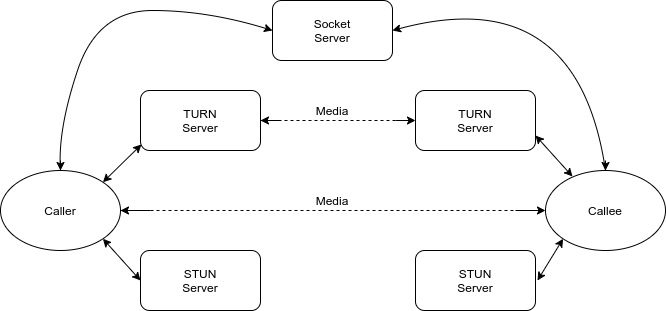
\includegraphics[width=0.5\textwidth]{images/WebRTCCommsArchitecture.png}
\end{figure}

Figure 3.2 displays the protocol used in communication to establish a call procedure composed of initiation, handshake, ICE negotiation, and hang-up stages which is used between peers.
In the first stage, initiation, peers are assigned to different rooms by the socket server when they first log in to the application. The purpose of these rooms are to send the status of communication for the users. This is useful because it sets the users up for the Idle step, in which they can receive or initiate calls. The processes of calling starts by registering with the room of the second/third/n peer to which that peer receiving a call. Should it be a case where the callee’s room is either empty or full, the process of calling is terminated. Should this not be the case, the incoming call is received. Only after the call is received is the WebRTC communication procedure started. 
\\The use of the WebRTC library is to send and receive media to or from peers. To begin, the peer initiates their media streams, this can either be audio, video, or both. On completion of this, and on ready of the streams, a peer connection is created by the callee, which is added to its local stream, subsequently creating an offer, and then finally sending this offer to the caller. The same procedure will be followed in the case of the text chat communication by taking the ready state of the peers media stream, without the media starting, and the application should start the data channel of text message transfer. On retrieval of this offer, the caller will create a peer connection. They will set a remote description, add the local stream of the offer, generate and answer and finally will send the answer to the callee. A remote description is set once the answer is received by the callee. ICE candidates are initiated only while a peer connection is set. If a local ICE candidate is generated, the protocol will verify the offer of creation, and will add the ICE candidates remote user. Should one of these checked items be available, the candidates local ICE is sent to the remote user, and subsequently will be added by the remote user as a remote ICE candidate.
\\On ready of local and remote streams, connection states of ICE are controlled. Should the state of ICE be in connected or completed, the call will be generated  and communication screens for audio and video will be presented to the users. If the ICE connection is in a checking or new state, the ICE protocol will wait and check the status periodically. Should this fail i.e the connection is in a different state, then the connection will be closed.
On call close, the connection and channel of data will be closed and all streams will be interrupted. This should terminate the callee’s room, and set the peers in a new state of ready to receive/create a new call.
\begin{figure}[h!]
    \caption{Communication Protocol between Peers.}
    \label{image:commsProtocol}
    \centering
    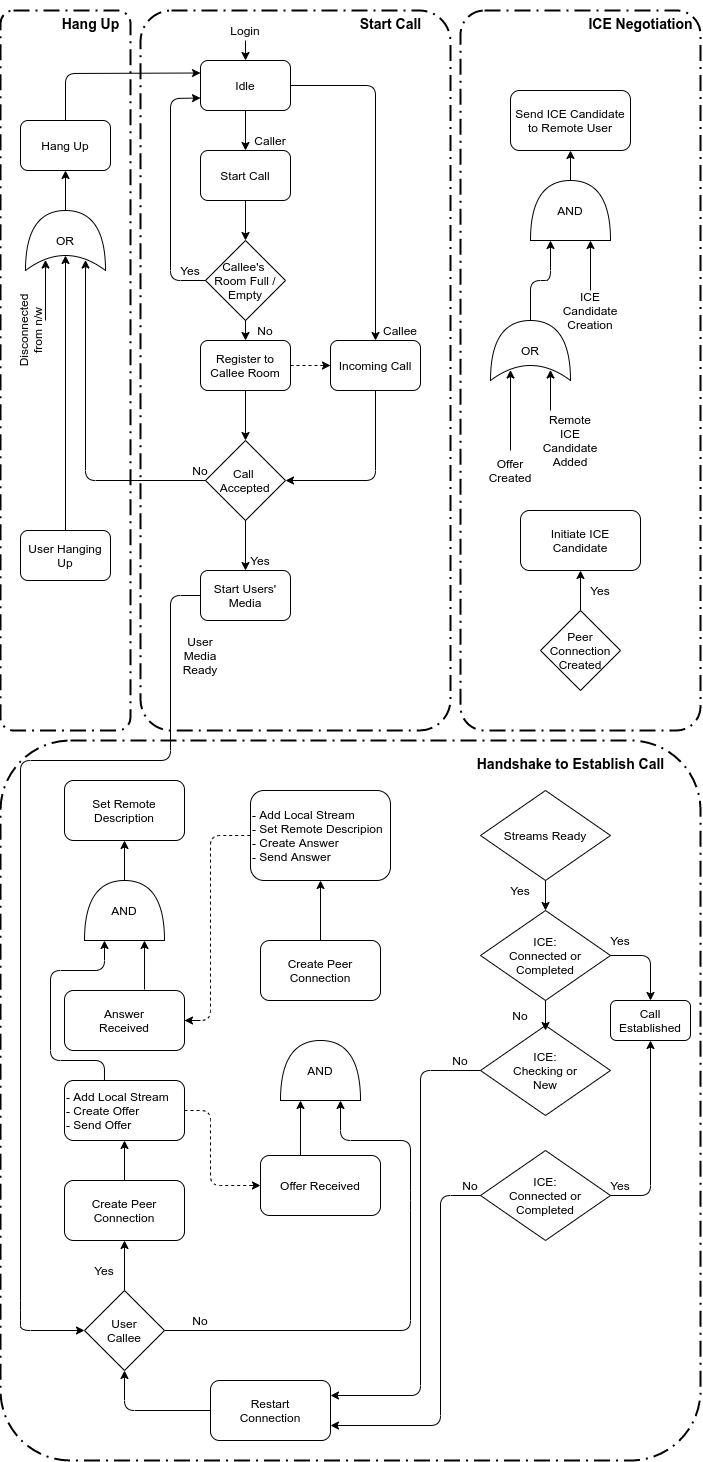
\includegraphics[width=0.8\textwidth]{images/CommunicationProtocol.png}
\end{figure}

